\chapter{Learning Ability Is a Life Lever}

A person who can learn whatever he needs has acquired a form of equipment that nature did not give him at birth.

This equipment is not a diploma. It is not the memory of school. It is not the ability to repeat correct phrases in conversation. It is the ability to meet a new problem, find the missing structure, practice the necessary movements, and eventually become competent where he was once helpless.

For wealth freedom, this ability is not decorative. It is central.

Capital changes. Markets change. Tools change. Professions change. The price of old skills changes. The value of new skills appears before most people recognize it. A person who can only use what he already knows will eventually be trapped by the depreciation of his existing abilities. A person who can learn keeps renewing the asset called himself.

This is why learning ability feels almost unfair. If one needs a skill and can learn it, he has more than a skill. He has a method for acquiring future skills. He owns a machine that can produce tools.

Most people want progress. That is rarely the problem. The problem is that wanting progress does not create progress. Many people spend a lifetime wanting to learn, planning to learn, talking about learning, and regretting not learning. At the end, they have proved only one thing: an ambitious heart is not enough.

\section*{A Simple Test}

How can a person judge his learning ability?

Education alone is a poor measure. Many people have received long schooling without learning how to learn. Many people have passed examinations without becoming capable practitioners. Many people have collected knowledge without turning it into action.

A more useful map has three levels:

\begin{enumerate}
\item You can learn what someone teaches you by hand.
\item You can learn what books, manuals, and tutorials teach.
\item You can learn what no one can teach you directly, and what no book yet explains systematically.
\end{enumerate}

\begin{center}
\begin{adjustbox}{max width=\linewidth}
\begin{tikzpicture}[node distance=0.65cm, every node/.style={font=\small, align=center}]
\node[draw, rounded corners, minimum width=3.1cm, minimum height=0.78cm] (one) {Level 1\\taught by hand};
\node[draw, rounded corners, minimum width=3.1cm, minimum height=0.78cm, right=of one] (two) {Level 2\\learned from texts};
\node[draw, rounded corners, minimum width=3.1cm, minimum height=0.78cm, right=of two] (three) {Level 3\\self-built path};
\draw[->] (one) -- (two);
\draw[->] (two) -- (three);
\end{tikzpicture}
\end{adjustbox}
\end{center}

The first level sounds easy, but many people do not pass it. They have been taught simple things repeatedly and still use them badly for decades. The issue is not always talent. Often it is attention, patience, and the willingness to think about details.

The second level is already rarer. It requires search, reading, comparison, judgment, and practice without a teacher standing beside you. It also requires the ability to choose better materials and discard poor ones.

The third level is the one that changes a life. It appears when the field is new, the opportunity is strange, the manuals are incomplete, and the experts either do not exist or cannot guide your particular path. At that level, you must build the route while walking it.

\section*{The Chopstick Problem}

A humble example is useful because it removes glamour.

Many people who believe they know how to use chopsticks are merely getting by. They can move food from bowl to mouth, but the tool is not stable, efficient, or natural. Because the task looks simple, they never inspect it. Because they can survive, they never learn it properly.

This is exactly how people fail in larger domains.

The key to using chopsticks is not mysterious. The lower chopstick stays still. The upper chopstick moves. The lower one must be stabilized by contact points in the hand; the upper one is controlled mainly by the thumb and index finger.

\begin{center}
\begin{adjustbox}{max width=\linewidth}
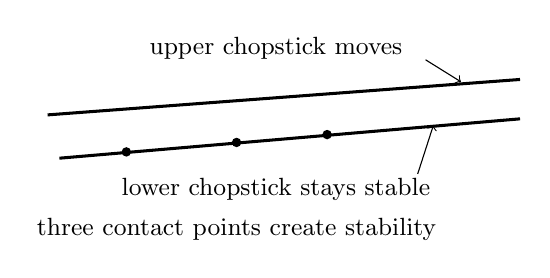
\begin{tikzpicture}[x=1cm,y=1cm, every node/.style={font=\small}]
\draw[line width=1.1pt] (0,0) -- (6,0.45);
\draw[line width=1.1pt] (0.15,-0.55) -- (6,-0.05);
\node[align=center] at (2.9,0.85) {upper chopstick moves};
\node[align=center] at (2.9,-0.95) {lower chopstick stays stable};
\draw[->] (4.8,0.7) -- (5.25,0.42);
\draw[->] (4.7,-0.75) -- (4.9,-0.13);
\fill (1.0,-0.47) circle (0.06);
\fill (2.4,-0.35) circle (0.06);
\fill (3.55,-0.25) circle (0.06);
\node[align=center] at (2.4,-1.45) {three contact points create stability};
\end{tikzpicture}
\end{adjustbox}
\end{center}

The decisive detail is often the direction of force from the ring finger. If the lower chopstick is not held against the hand in the right direction, it wobbles. Once that detail is corrected, the remaining practice is short: move the upper chopstick, open and close, pick up small objects, repeat until the hand stops resisting.

The example matters because it reveals several facts.

First, a simple skill may contain a hidden key. Second, the hidden key is usually discovered by careful observation, not by impatience. Third, many people who can perform a skill cannot teach it, because they never found the key consciously. Fourth, once a key is found, a problem that has irritated someone for years may be solved in minutes.

This is a serious lesson disguised as a small domestic skill.

\section*{Teaching as Examination}

The best test of whether you truly understand a skill is whether you can teach it to another person.

When you learn only as a student, you can lower your standard without noticing. You may think, ``I understand,'' when you can merely follow. You may think, ``I can do it,'' when you can only do it under familiar conditions. You may think, ``This is obvious,'' when you have never explained it to someone who does not yet see the structure.

Teaching exposes the gap.

To teach well, you must know where the learner fails. You must distinguish the surface movement from the core mechanism. You must identify the smallest necessary correction. You must choose the right order. You must observe whether your explanation changes behavior. If it does not, you must improve the explanation instead of merely getting angry.

This is why teaching upgrades learning. If, while learning a skill, you keep asking how you would teach it later, your own attention becomes sharper. You look for structure. You separate key points from noise. You ask better questions:

\begin{enumerate}
\item What is the central mechanism?
\item Why do competent people do it well?
\item Where do beginners usually fail?
\item Which practice is unavoidable?
\item What small correction produces the largest improvement?
\end{enumerate}

These questions work for chopsticks, writing, investing, programming, sales, public speaking, and almost every practical skill.

The position you occupy changes what you see. A learner sees difficulty. A teacher must see mechanism. A practitioner sees feedback. An investor sees risk, time, and position. Move to a higher position, and the same problem often becomes a different problem.

\section*{The Price of Avoiding Trouble}

A large part of human stagnation can be explained by one sentence:

\begin{quote}
I know I should do it, but it is too much trouble.
\end{quote}

This sentence looks harmless. It is not.

The trouble avoided today often becomes repeated trouble tomorrow. A person who refuses to spend a short time learning chopsticks may suffer small embarrassment at every meal. A person who refuses to learn basic accounting may lose money quietly for years. A person who refuses to learn how investment accounts, taxes, and risk controls work may remain permanently outside the world where capital can work for him. A person who refuses to learn writing may keep losing chances to clarify thought, persuade others, and create durable value.

The choice is not between trouble and no trouble. The choice is usually between brief trouble and lifelong trouble.

\begin{center}
\begin{adjustbox}{max width=\linewidth}
\begin{tabular}{p{0.36\linewidth}p{0.48\linewidth}}
\hline
Choice & Consequence \\
\hline
Learn through short trouble & The skill becomes part of you. \\
Avoid short trouble & The same weakness repeats for years. \\
Record practice & Improvement becomes visible. \\
Only think about practice & The old route returns in the morning. \\
\hline
\end{tabular}
\end{adjustbox}
\end{center}

This is why time records are powerful. When a person writes down how the day was actually spent, fantasy weakens. The record often says, plainly, ``I was busy, but not on the work that matters.'' This can be discouraging, but it is also useful. It turns vague dissatisfaction into data.

Thinking about a thousand routes at night is not the same as walking one route in the morning. Only time used in action moves the person.

\section*{Learning from Texts}

If every useful skill required someone to teach us by hand, a lifetime would be too short.

People with valuable skills are busy. Many cannot teach. Some do not know how they do what they do. Some can demonstrate but cannot explain. Some are unwilling. Even those who are willing may not appear at the moment you need them.

Therefore, the second level of learning is essential: learn from books, manuals, papers, tutorials, documentation, and examples.

This level has three subskills.

First, you must be willing to search widely. One article is rarely enough. One video is rarely enough. One recommendation list is not a method. You need the patience to inspect many sources and notice which ones explain the structure better.

Second, you must judge quality. A simple beginner rule for books is still useful: prefer reputable publishers, repeated editions, and works that have survived use by many serious readers. This rule is not perfect, but it is far better than feeding the mind whatever is most convenient.

Third, you must practice what the text teaches. Reading without use produces the illusion of growth. The sentence is understood, but the behavior is unchanged. The manual has been consumed, but the skill has not entered the body.

The second level is where many adults should spend much more time. The world's accumulated knowledge is not hidden. Much of it is inexpensive. Some of it is free. The scarce part is not access; it is the ability to turn access into ability.

\section*{The Third Level}

The third level begins when available instruction is insufficient.

This may happen because a field is new. It may happen because your combination of problems is unusual. It may happen because the best knowledge is scattered across several disciplines. It may happen because everyone around you is still using old categories to look at a new thing.

At this level, no one can provide the complete route. You must construct it.

A useful operating sequence is:

\begin{enumerate}
\item define a strong reason to learn the skill;
\item find the minimum necessary knowledge;
\item ask repeatedly, ``Where is the key point?'';
\item begin using the skill immediately;
\item trust practice enough to keep going;
\item record practice so progress becomes measurable;
\item organize new concepts and connect them clearly;
\item protect your time from useless argument.
\end{enumerate}

The last item matters more than it first appears. At higher levels of learning, many discussions are not helpful. They consume attention, provoke ego, and create the feeling of work without producing progress. Listening broadly is useful. Considering a few good opinions is useful. But the final decision and the final path must be your own.

This is not a slogan of heroic individualism. It is an operational necessity. If the path already existed clearly, you would be at the second level. At the third level, your ability to find or build your own path is the test itself.

\section*{A New Asset Before the Books}

An early encounter with Bitcoin is a good example of third-level learning. This is not a recommendation to buy an asset because it is mentioned here. The rule remains simple: do not invest in what you do not understand.

The example is about learning.

In the early years, there was no mature curriculum, no shelf of reliable books, no patient teacher who could guide an ordinary learner step by step. There was a white paper, some code, scattered discussions, and a strange object that seemed absurd to most people. To understand it, one had to touch mathematics, cryptography, distributed networks, incentives, finance, programming, hardware, security, politics, sociology, and psychology. Few people had formal training in all of these. Many had formal training in none.

That situation could not be solved by waiting for a teacher.

A person who wanted to understand had to build a private university around the problem. Read a little, test a little, ask, search, compare, make mistakes, revise, connect one discipline to another, and continue. Over years, the learner would not merely understand one asset better. He would become a different learner.

This is one reason strange opportunities are valuable even before their financial result is known. They may force a person into a higher mode of learning. They may teach him to cross boundaries. They may reveal that the world is not divided according to school subjects, and that important opportunities often live between categories.

The financial return of an asset may be large or small. The return on becoming able to learn such an asset can be larger still.

\section*{Logic as Self-Rescue}

Another path into the third level may begin with embarrassment.

Imagine being persuaded by one person in the afternoon, then persuaded by another person later, and realizing at night that their views contradict each other. Both cannot be right. Yet both felt convincing. The frightening discovery is not that one of them was wrong. The frightening discovery is that your own mind could be carried in opposite directions without noticing.

This is the moment when logic stops being a school topic and becomes self-rescue.

A person in that position may begin searching for books on thinking, critical thinking, argument, evidence, and reasoning. He may discover that clear thinking has methods. He may also discover that reading the methods is easier than practicing them.

Logic is socially expensive. Careful reasoning often irritates people. Few enjoy having their contradictions exposed. Few welcome evidence that their thinking is weak. Even close friends may become defensive when a discussion becomes too precise. Therefore, the practice of reasoning cannot depend too much on pleasant discussion. It must become a private discipline: read, write, test, revise, notice fallacies, separate emotion from inference, and keep doing it.

Here again, the third level appears. No teacher can live inside your judgment. No book can make your next thought careful by itself. You must operate the tool.

\section*{Learning Creates Luck}

People often call a successful learner lucky. Sometimes they are right, but not in the way they think.

Luck is not fully controllable. But a person can create more surfaces on which luck can land. Learning does exactly that.

Every useful concept in the mind can connect with another concept. The more organized concepts you have, the more possible connections exist. Some connections will be expected. Others will be surprising. The surprising ones often feel like luck: a skill learned for one purpose becomes useful elsewhere; a book read years ago explains a current problem; a technical detail from one field reveals an opportunity in another; a practice that once seemed unrelated becomes decisive.

Without concepts, there is little to connect. Without practice, the concepts remain weak. Without organization, they cannot be found when needed.

\begin{center}
\begin{adjustbox}{max width=\linewidth}
\begin{tikzpicture}[node distance=0.72cm, every node/.style={font=\small, align=center}]
\node[draw, rounded corners, minimum width=2.55cm, minimum height=0.75cm] (learn) {learn\\concepts};
\node[draw, rounded corners, minimum width=2.55cm, minimum height=0.75cm, right=of learn] (use) {use\\them};
\node[draw, rounded corners, minimum width=2.55cm, minimum height=0.75cm, below=of use] (connect) {new\\connections};
\node[draw, rounded corners, minimum width=2.55cm, minimum height=0.75cm, left=of connect] (luck) {created\\luck};
\draw[->] (learn) -- (use);
\draw[->] (use) -- (connect);
\draw[->] (connect) -- (luck);
\draw[->] (luck) -- (learn);
\end{tikzpicture}
\end{adjustbox}
\end{center}

A person who learns widely and practices seriously will often say, ``I never expected this would be useful here.'' That sentence is the sound of learning becoming luck.

\section*{The Knife Before the Wood}

The phrase ``learn, learn learning, then learn'' is not repetition for emphasis. The middle word is the object. First learn how learning works; then learn the particular thing.

This is sharpening the knife before cutting wood.

Sharpening does not replace cutting. Methodology does not replace practice. But a dull knife wastes strength, and poor learning methods waste life. A person who knows how to find minimum necessary knowledge, how to identify the key point, how to practice deliberately, how to record progress, how to teach as a test, and how to build a path when no complete path exists, will cut through more material with less confusion.

Learning ability also repairs one's relationship with age. After thirty, a sincere lifelong learner often feels embarrassed by his past self. Problems that once seemed impossible now look simple. This does not mean the past self was stupid in some absolute sense. It means the present learning system is stronger. The old difficulty was real under the old system.

This realization should make us humbler and more hopeful at the same time.

Humbler, because today's certainty may later look crude.

More hopeful, because tomorrow's self may be able to solve what today's self cannot yet solve.

\section*{Your Own Crossing}

No one can prescribe the exact crossing for another person.

One person enters third-level learning through logic. Another through programming. Another through investing. Another through writing, design, business, parenting, science, or a strange new technology. Each path contains different materials, different bottlenecks, and different emotional costs.

But the general principle is stable:

\begin{quote}
You must eventually discover how you cross from being taught to teaching yourself.
\end{quote}

This principle is also one of the deepest principles of investing. In the end, your road must be walked by you. You can listen to many people. You can study a few carefully. You can borrow frameworks, rules, and warnings. But no one else can replace your judgment, your risk, your time horizon, your emotional discipline, or your responsibility.

Once you have succeeded even once at the third level, life changes. You become less afraid of unfamiliar fields. You no longer assume that absence of a teacher means impossibility. You no longer worship existing paths. You know that clumsiness can be temporary, books can be partial, experts can be absent, and still a route can be built.

That confidence is not empty confidence. It is earned from crossing.

\section*{Practice}

Choose one small skill you already think you know. If possible, choose something ordinary enough that vanity cannot hide inside it: chopsticks, handwriting, typing, explaining a concept, keeping a daily time record, making a simple spreadsheet, reading a manual, or writing a clear paragraph.

Then do three things.

First, inspect the mechanism. Where is the key point? What do competent people actually do? What do beginners usually miss?

Second, teach it to someone else, or write instructions as if you had to teach it. If the instruction fails, improve the instruction. Do not blame the learner too quickly.

Third, record the practice. Not forever, perhaps, but long enough to see whether attention is becoming action.

The purpose is not the small skill itself. The purpose is to train the ability beneath the skill.

A person who refuses small trouble will be ruled by repeated trouble. A person who learns from small trouble installs a method. That method becomes equipment. Equipment becomes leverage. Leverage, applied over time, becomes freedom.
